
\input{pre} 

\begin{document}

\begin{frame}
\titlepage

\end{frame}

\section{Fieldtrip}
\begin{frame}{Fieldtrip}
\begin{itemize}
    \item Who: Samira Verhees and Chiara Naccarato
    \item When: 1 -- 9 August 2019
    \item Where: Botlikh district, Daghestan
    \item Aims: collect a survey on the agreement patterns of ordinal numerals, translate texts recorded by T.E. Gudava \citep{gudava1962}, collect some lexical data (Swadesh lists)
    \pause
    \item Additional tasks: find more consultants to work with, collect some preliminary observations on the sociolinguistic situation in Botlikh and Miarso
\end{itemize}
\end{frame}

\begin{frame}
\begin{center}
    \begin{huge} \color{darkscarlet}
    Background on the language and village(s)
    \end{huge}
\end{center}
\end{frame}

\section{Language}
\begin{frame}{The Botlikh language}
\begin{itemize}
    \item Botlikh > Andic group > East Caucasian language family
    \item Unwritten
    \item \textasciitilde{}5000-8000 speakers
    \item Mostly spoken in 4 villages in northwestern Daghestan:\footnote{\footnotesize{Population figures from the 2010 census, accessed via the Russian Wikipedia pages of the respective villages.}}
    \begin{itemize}
        \item Botlikh (main village) - pop. 12.159
        \item Miarso (founded as \textit{khutor} several hundred years ago) - pop. 1714
        \item Ashino (small khutor) - pop. 79
        \item Ankho (even smaller khutor not mentioned by consultants) - pop. 35
    \end{itemize}
\end{itemize}
\end{frame}

\begin{frame}{The Botlikh language}
\begin{itemize}
    \item Each village has its own dialect %except Ankho?
    \item Speakers distinguish between them, but they are fully mutually intelligible
    \item Opinions vary on the language's vitality --- it is still passed on to children and spoken at home, but some families/children are shifting to Russian
    \item Direct neighbors of Botlikh include other Andic languages (Andi, Karata, Godoberi) and Avar %Botlikhs understand Godoberi to a certain extent, but not Andi
\end{itemize}
\end{frame}

\begin{frame}{Botlikh on the map}
\begin{figure}[h]
\centering
\fbox{\includegraphics[scale=0.4]{images/globalmap.png}}
\end{figure}
\end{frame}

\begin{frame}{Botlikh on the map}
\begin{figure}[h]
\centering
\fbox{\includegraphics[scale=0.3]{images/hood.png}}
\end{figure}
\end{frame}

\section{Village}
\begin{frame}{The village}
\begin{itemize}
    \item Botlikh is the administrative center of the eponymous district, which was formed in 1929
    \item Already in the 19th century, Botlikh had become an important trading center, which, according to \citep[59]{wixman1980} slowed down the assimilation of Botlikhs by Avars 
    \item Contemporary Botlikh is fairly urbanized: there is a decent road from Buinaksk / Makhachkala to Botlikh and there are a lot of shops and other facilities (e.g. a hospital, a hotel, and even a sushi restaurant)
    
\end{itemize}
\end{frame}


\section{Village}
\begin{frame}{The village}
\begin{itemize}
\item The village consists of two distinct parts: the ``old village'' and the \textit{mikrorayon} --- a sort of suburb built in the 1970s to house the employees of a new factory % In 1972 the school was built, some houses and the hospital. In 1975 the factory "Progress" (a military factory) was completed and workers started coming to Botlikh. In 1980 the main buildings were completed.
\item Most ethnic Botlikhs live in the old village, while Avars and other Andic people tend to live in the Mikrorayon
\item Botlikhs have garden plots outside the old village centre, where they grow fruit trees like apricots, peaches, etc. but also vegetables, corn, pumpkins
\item Cattle breeding is less common and in decline
\end{itemize}
\end{frame}

\begin{frame}{Map of the village}
\begin{figure}[h]
\centering
\fbox{\includegraphics[scale=0.3]{images/botlikh.png}}
\end{figure}
\end{frame}

\begin{frame}{Language use in the village}
\begin{itemize}
    \item Botlikh is used at home and by Botlikhs among each other
    \item Avar, Russian and Botlikh are all used for interethnic communication, so there is L2 speaker input into Botlikh and code mixing
    \item Avar was historically an important lingua franca (used in communication with neighbors), and Botlikhs have been subsumed under Avars during census since the 1930s
    \item Many Botlikhs still consider themselves ``a type of Avars'', though there is a small movement of Botlikh patriots who advocate for the recognition of Botlikh as a separate ethnic group
\end{itemize}
\end{frame}
    
\begin{frame}{Language use in the village}
\begin{itemize}
    \item Russian is currently gaining dominance at the expense of Avar as L2
    \item Children at kindergarten speak mostly Russian
    \item There are two opposing attitudinal tendencies regarding language use at home: some families promote the use of Russian by children, because they associate it with upward social mobility, while others make a point of speaking only Botlikh at home, because they value the preservation of their native language
\end{itemize}
\end{frame}

\begin{frame}{Language use by children}
\begin{figure}[h]
\centering
\fbox{\includegraphics[height=6cm]{images/madina.JPG}}
\end{figure}
\end{frame}


\begin{frame}{Language use in the family}
\begin{itemize}
    \item Mixed marriages with other local people, as well as Russian wives, are quite common
    \item Interestingly, in case of mixed marriages women are not required to learn the language of their husband, and they pass on their native language to the children
    \item (A mixed Andi-Godoberi couple who live in Botlikh reported that they speak Avar to each other, while each speaks to the children in their own native language)
\end{itemize}
\end{frame}


\begin{frame}{The old village}
%The old village is divided into quarters: we recorded some toponyms and coordinates, but very haphazardly.
\begin{figure}[h]
\centering
\fbox{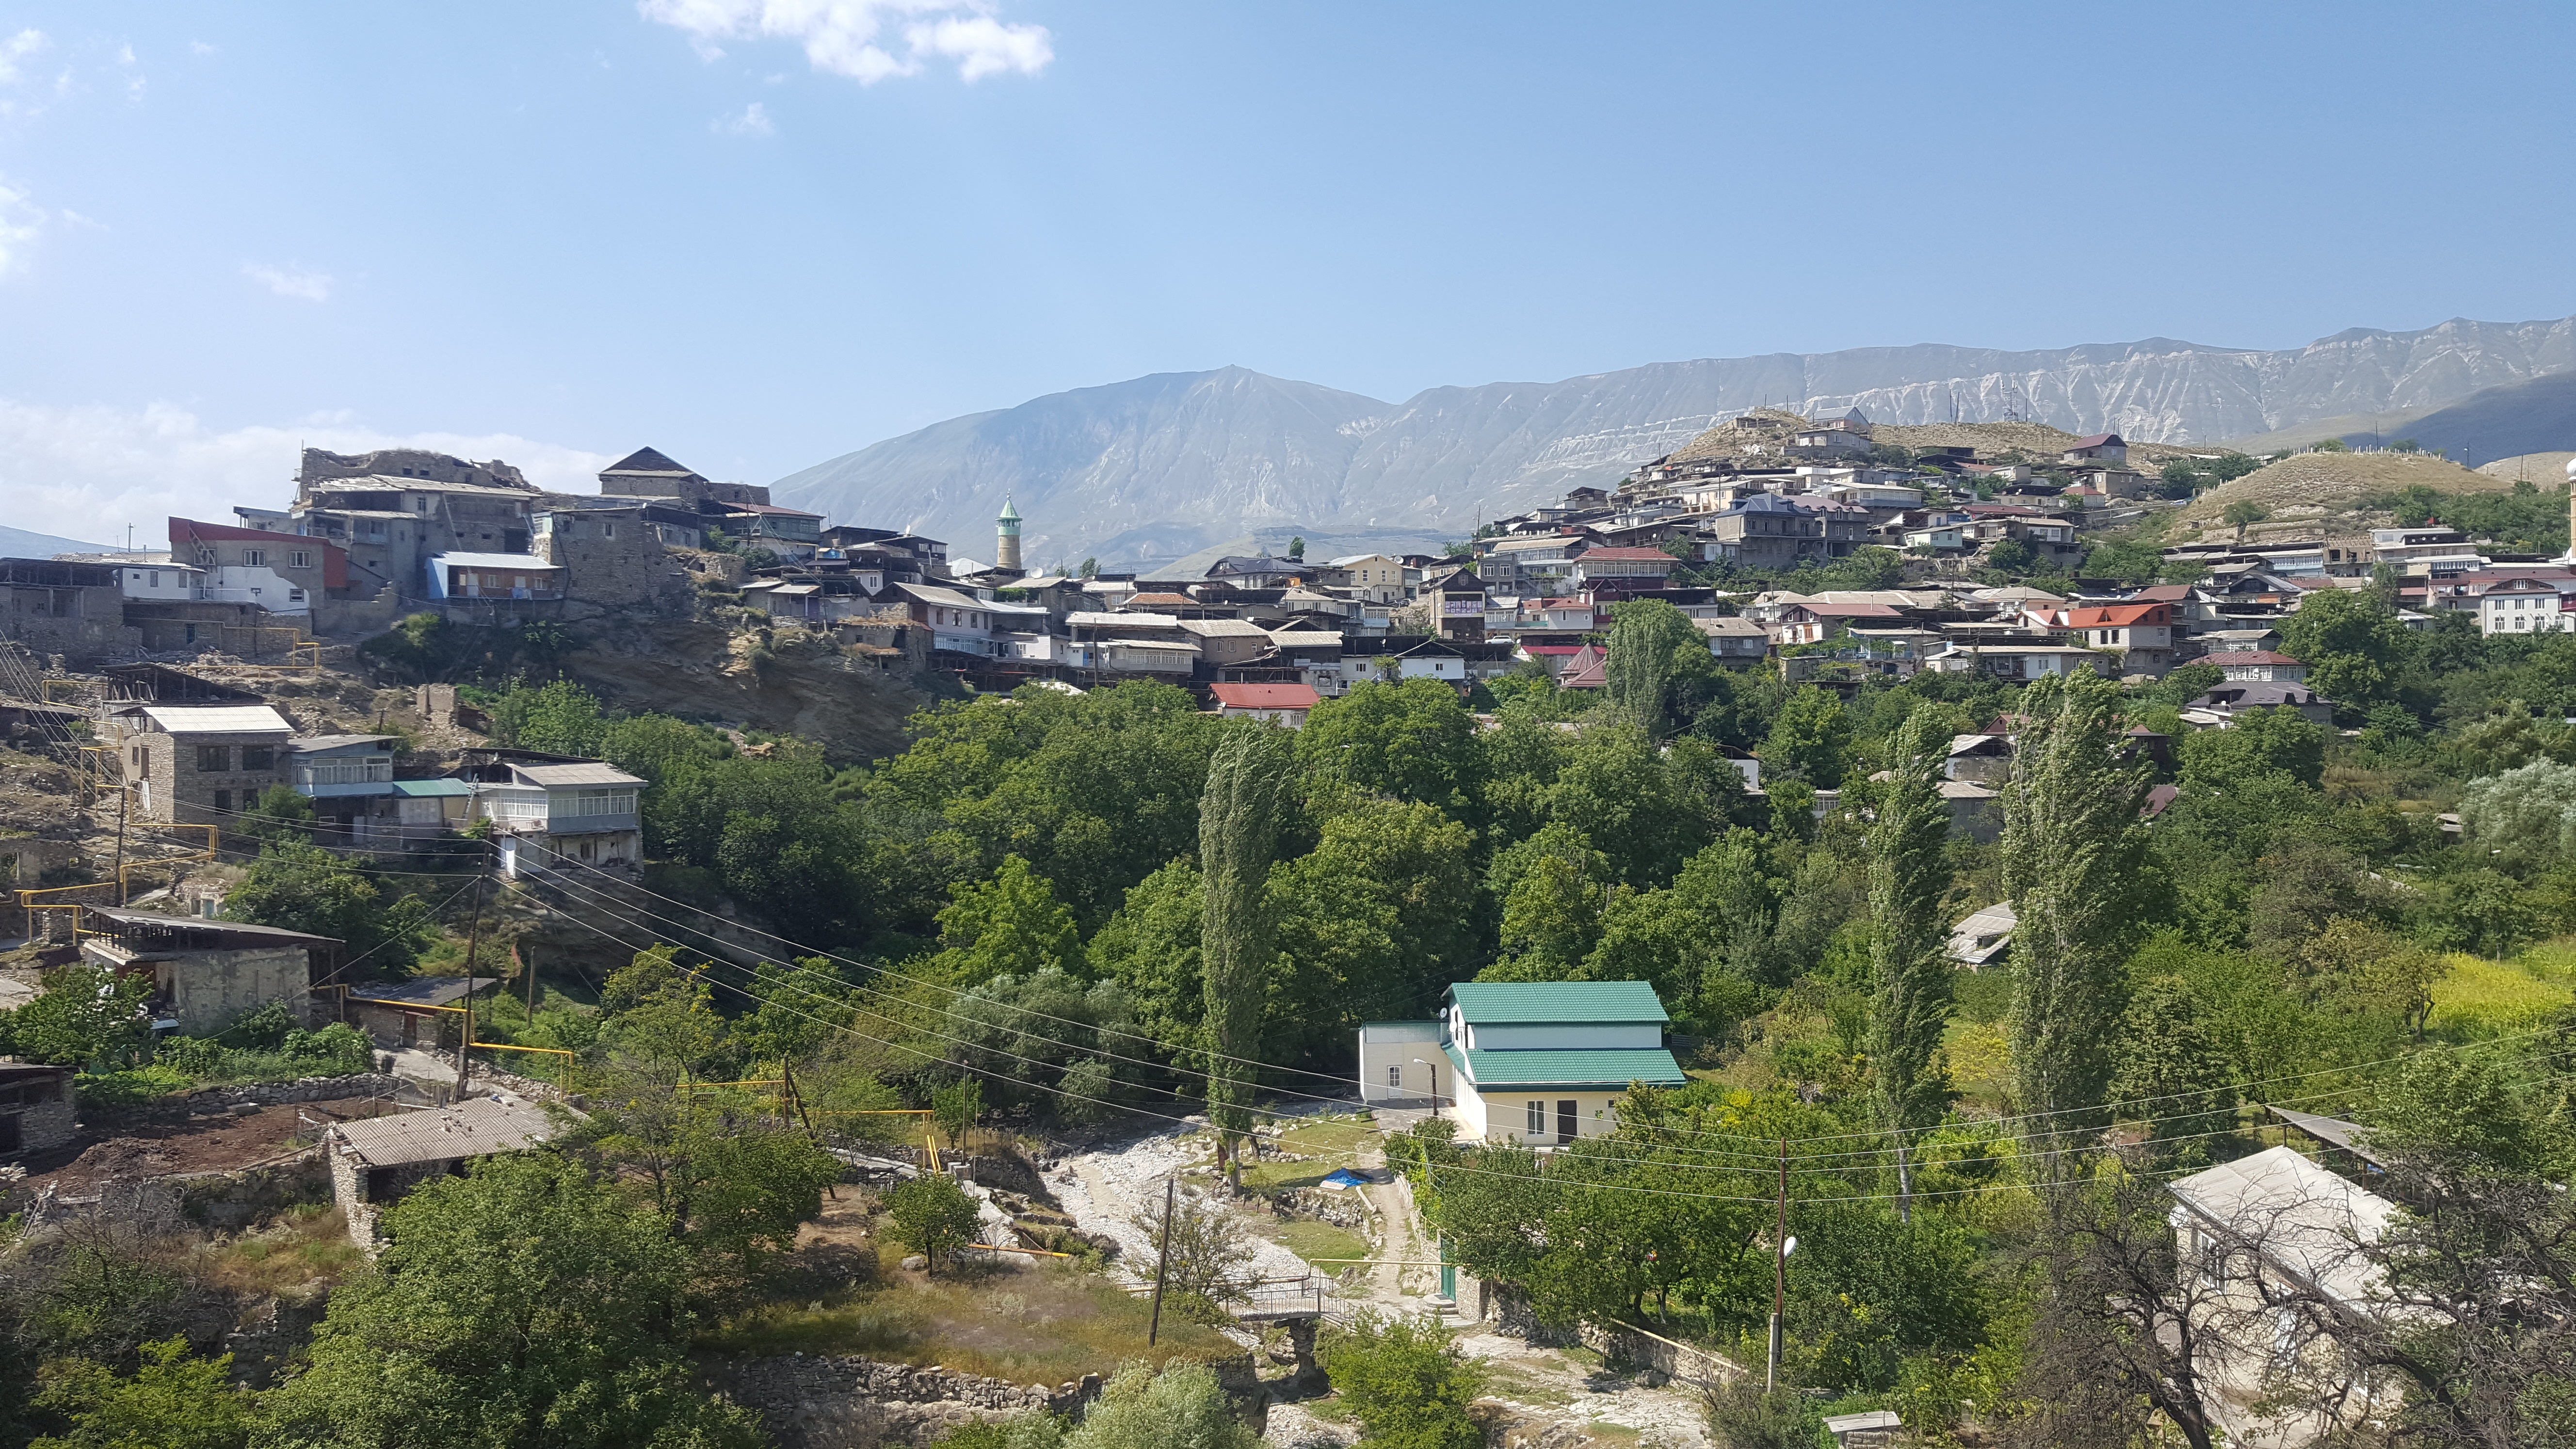
\includegraphics[height=6cm]{images/old_village.jpg}}
\end{figure}
\end{frame}

\begin{frame}{The old village}
\begin{figure}[h]
\centering
\fbox{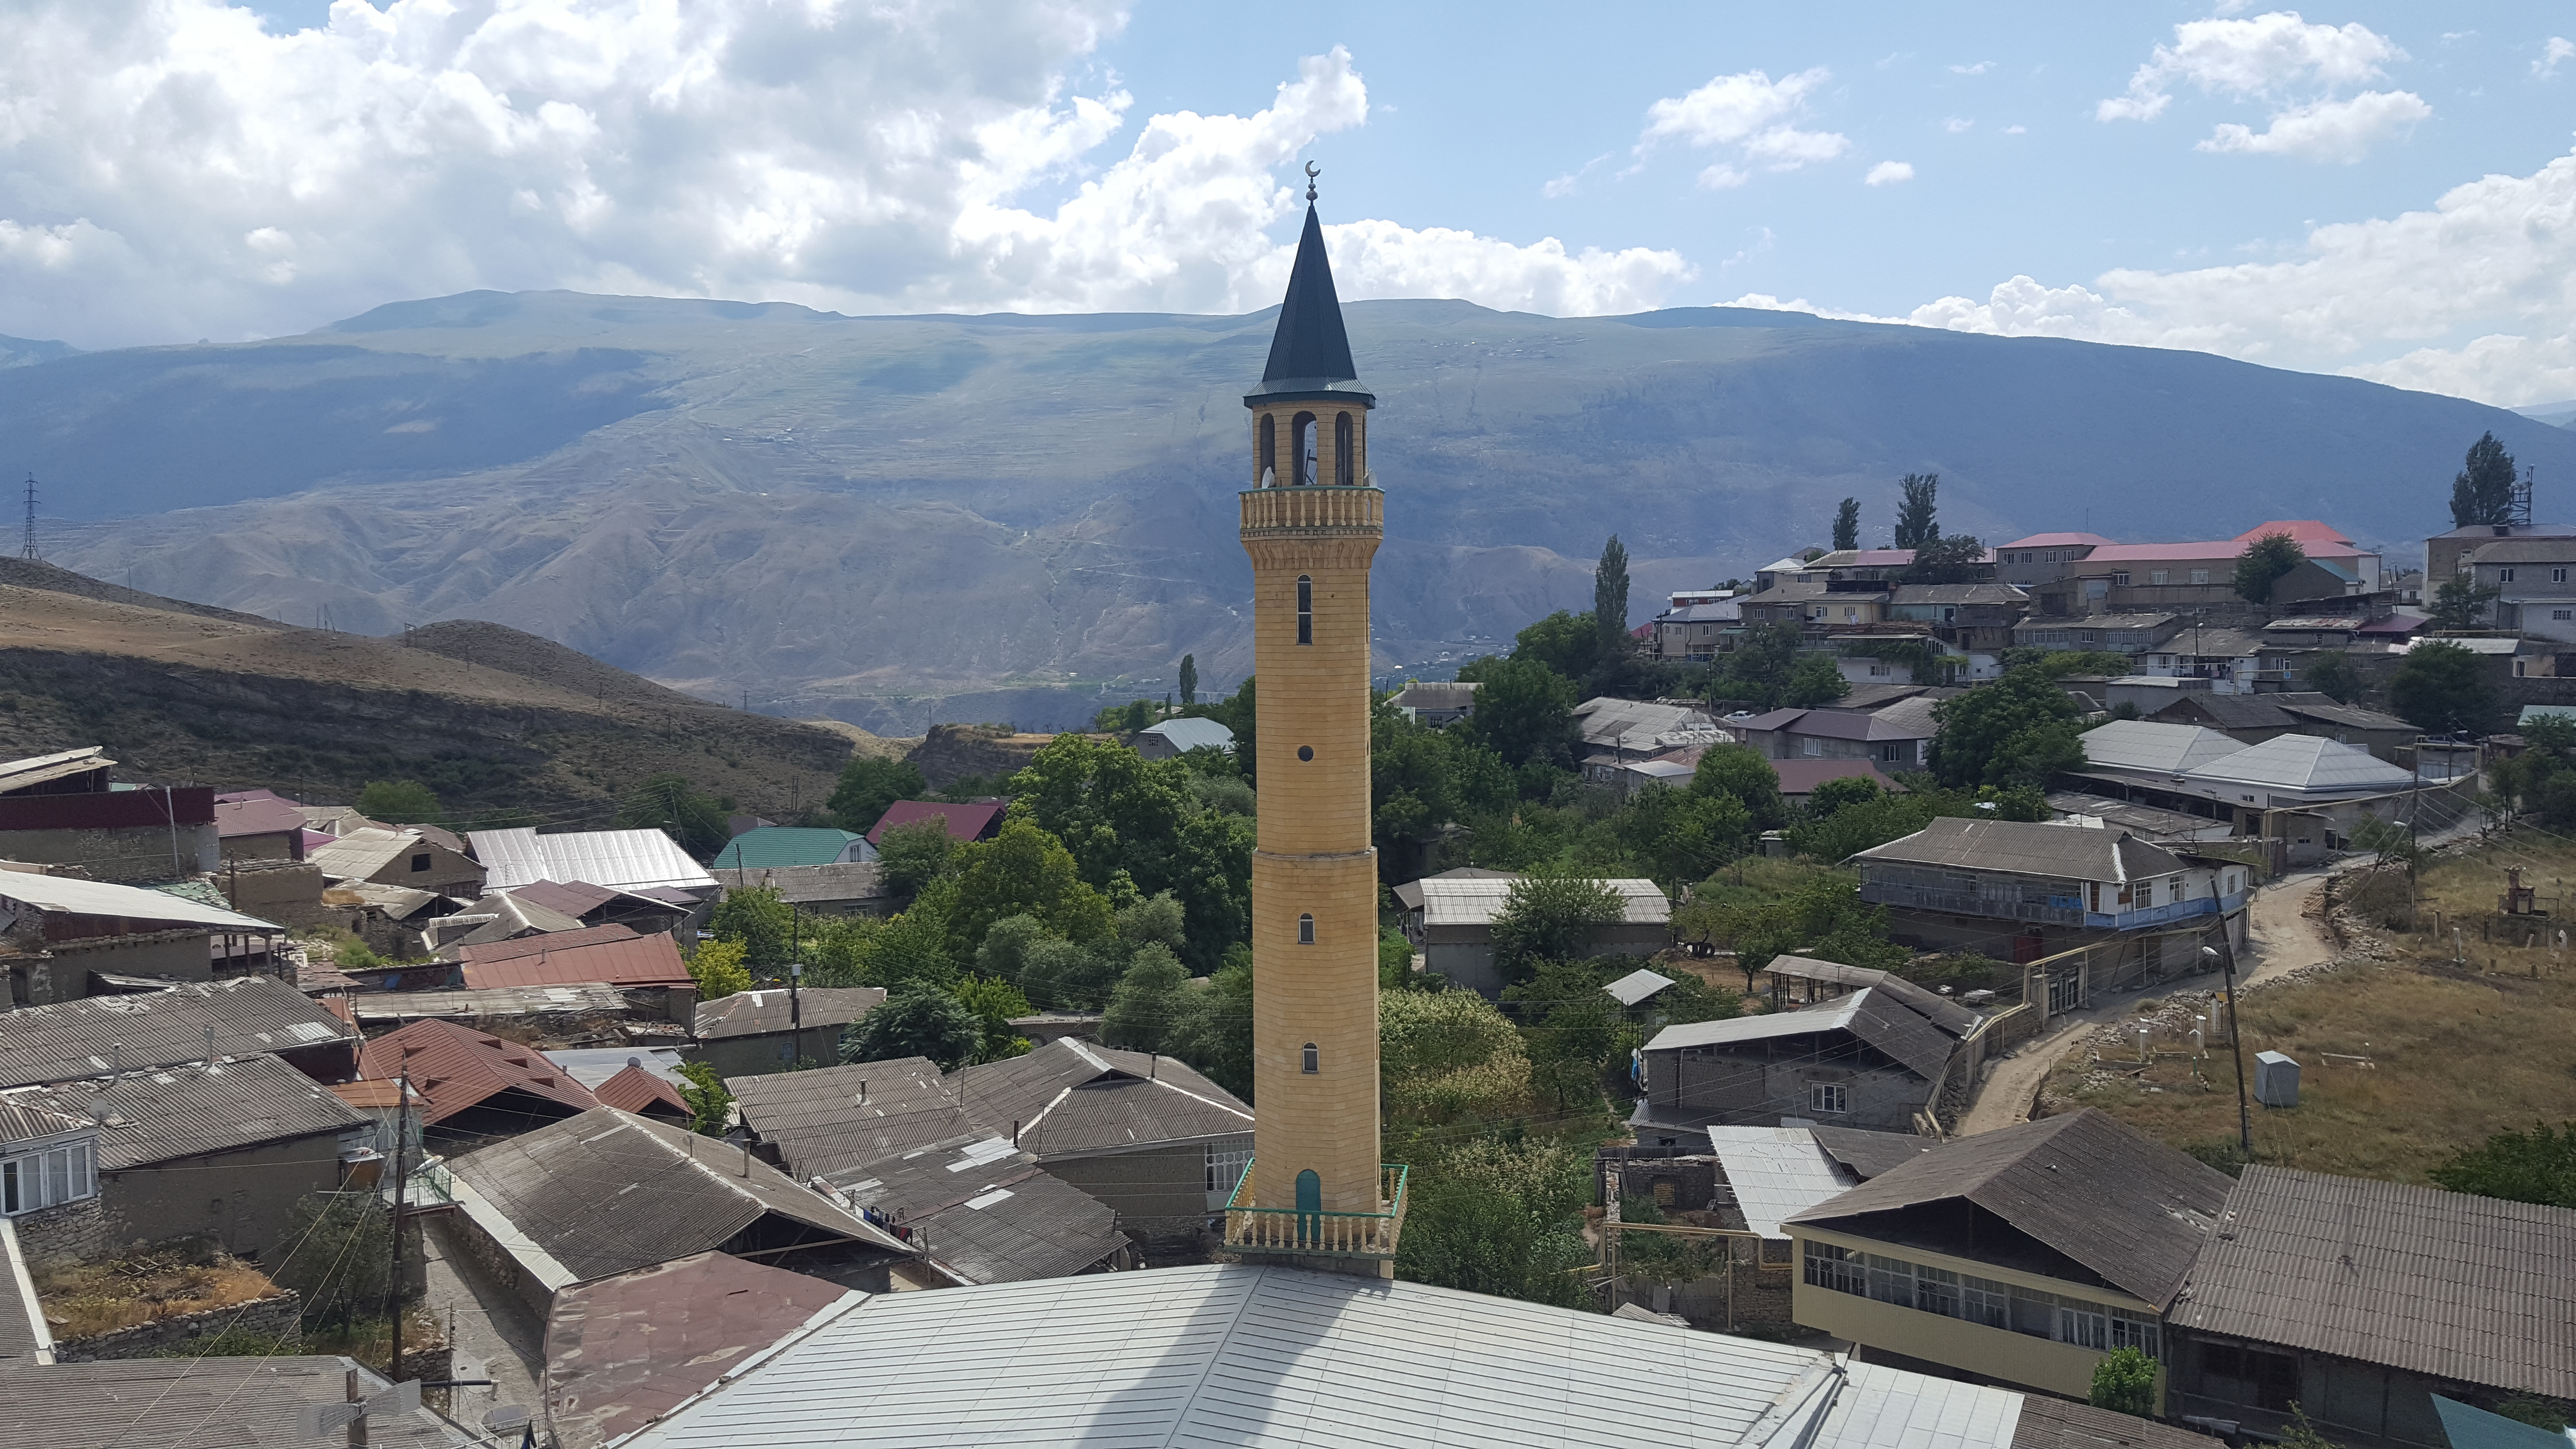
\includegraphics[height=6cm]{images/old_village2.jpg}}
\end{figure}
\end{frame}

\begin{frame}{The old village}
\begin{figure}[h]
\centering
\fbox{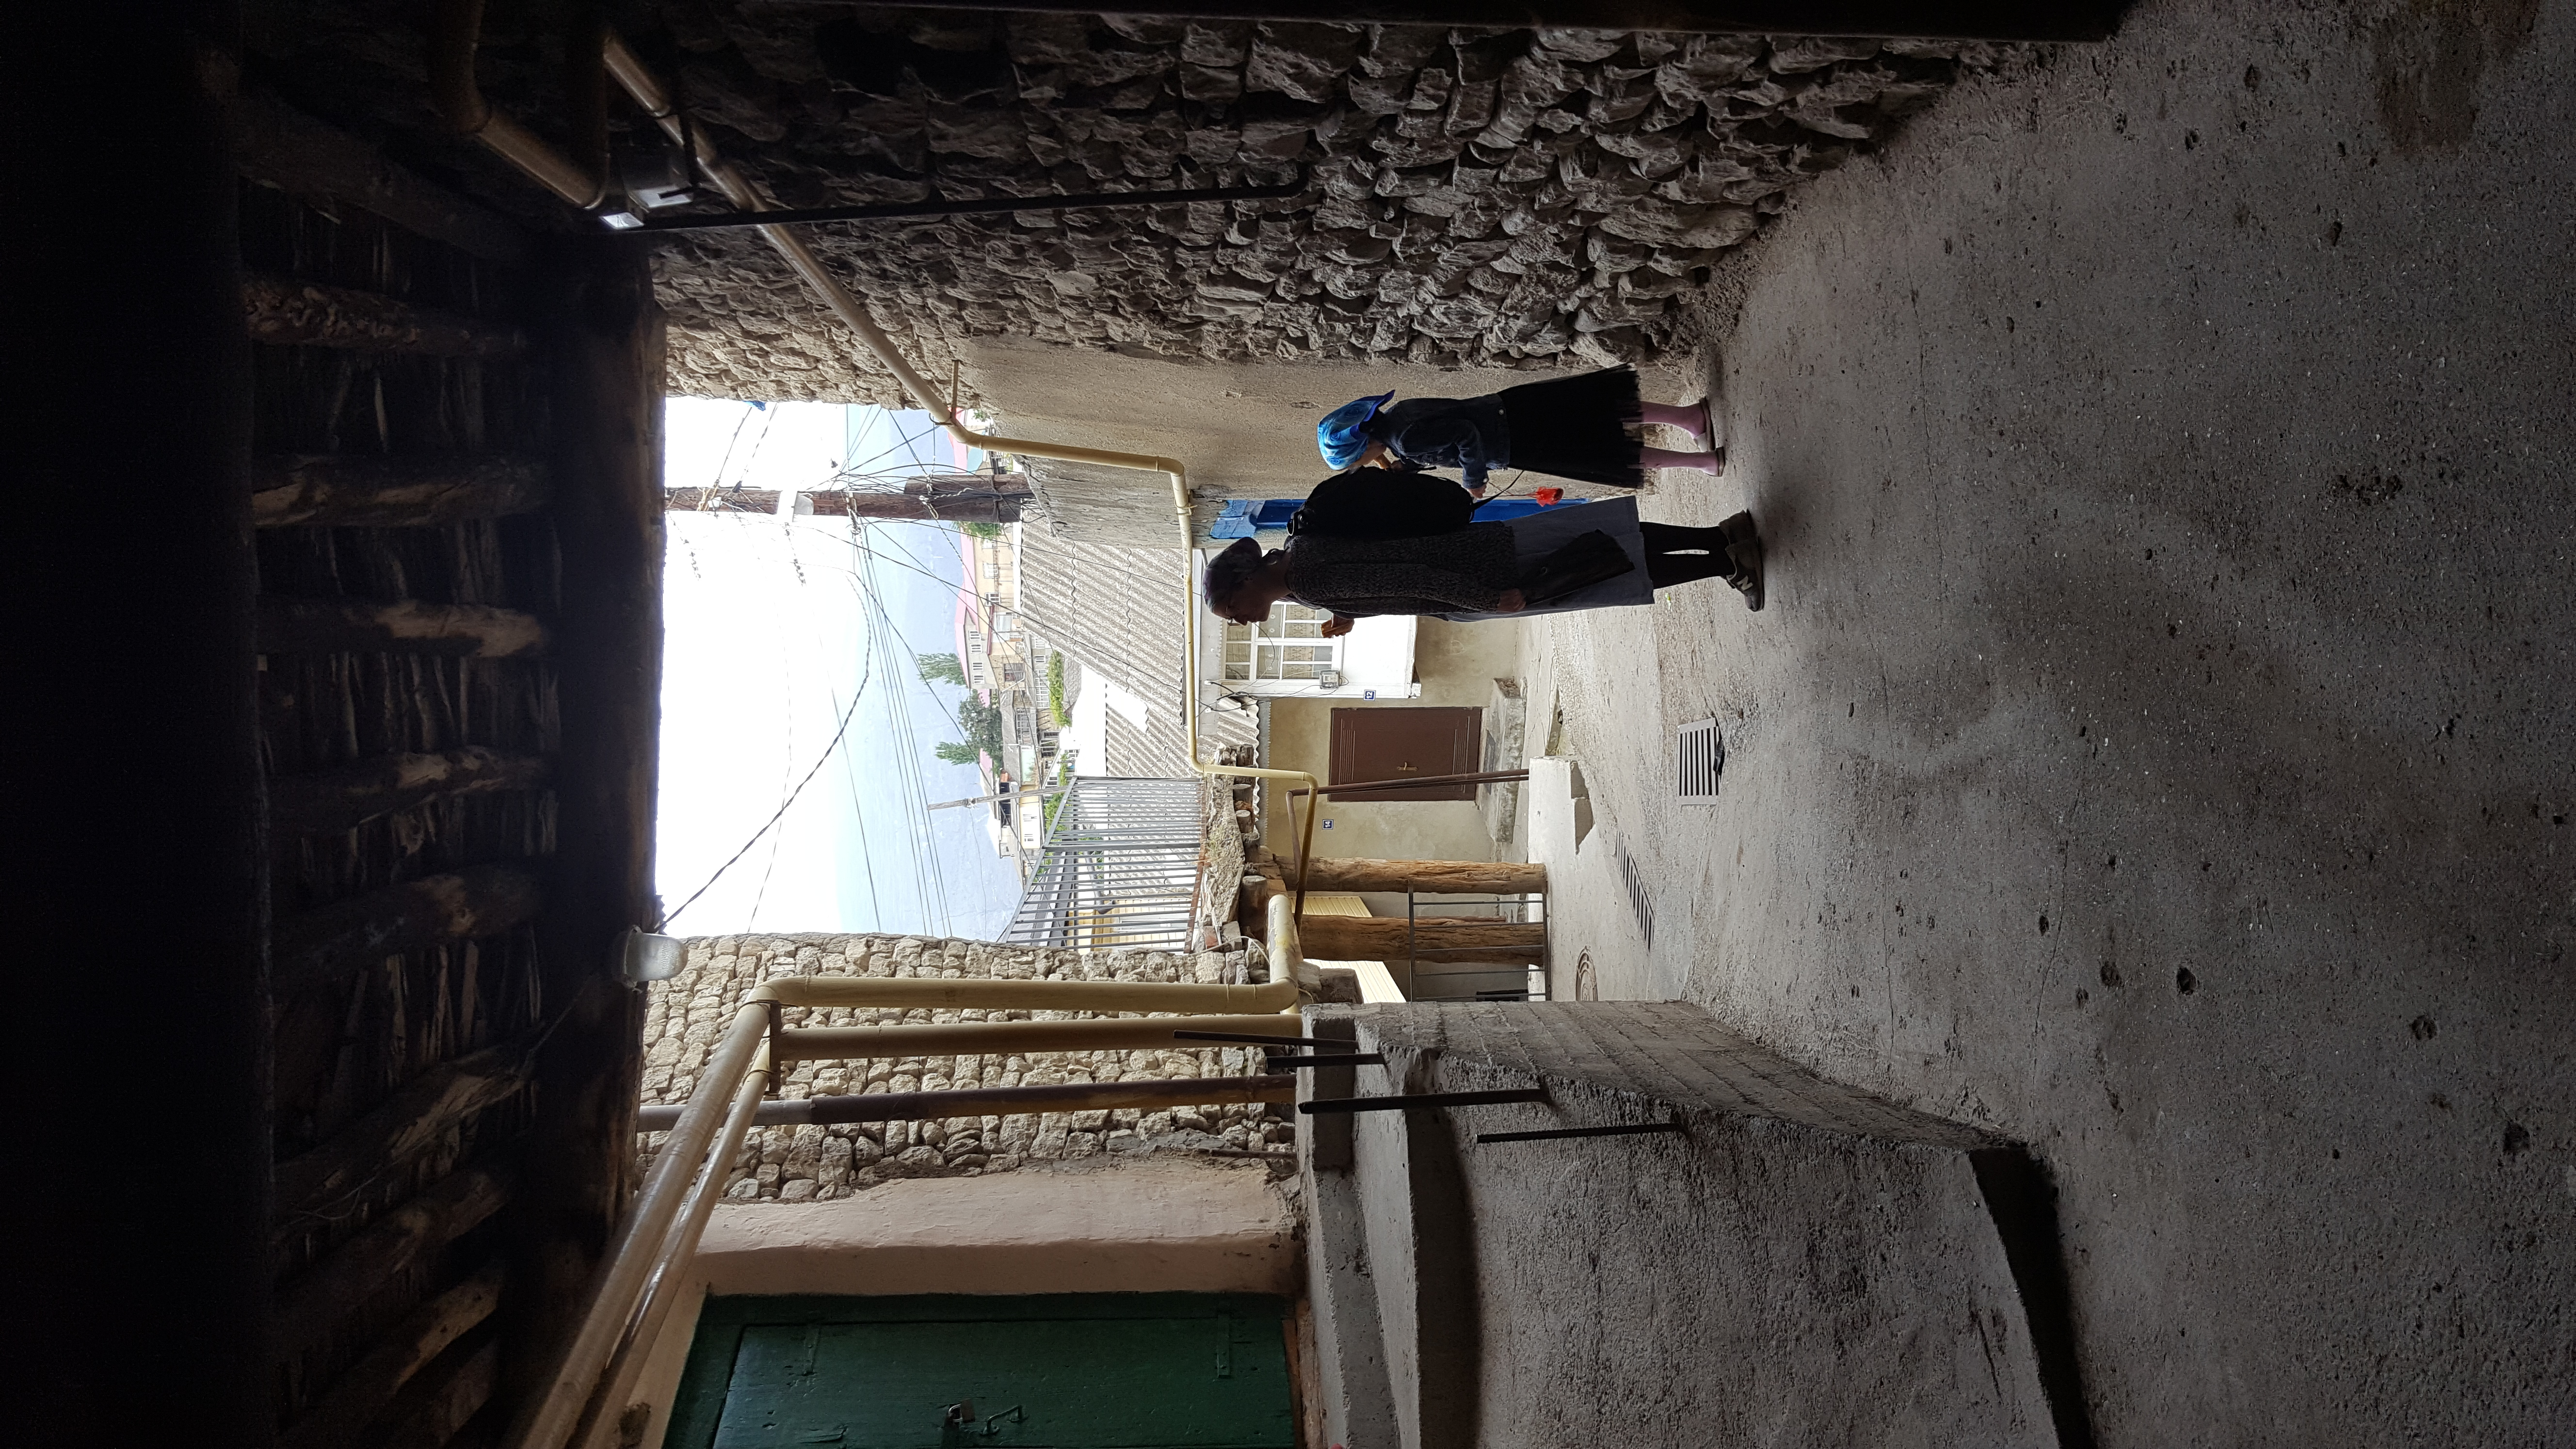
\includegraphics[height=4cm, angle=-90]{images/tunnel.jpg}}
\end{figure}
\end{frame}

\section{Miarso}
\begin{frame}{Miarso}
 \begin{itemize}
    \item Founded as a khutor either \textasciitilde{}200-250 or \textasciitilde{}500-600 years ago
    \item Population: between \textasciitilde{}1700 and \textasciitilde{}2500
    \pause
    \item \textasciitilde{}20 minutes from Botlikh on foot
    \item Other close villages: Godoberi, Ansalta, Tando, Rakhata, Shodroda
    \item People from Godoberi and villages in the Tsumadinsky district used to stop in Miarso on their way to the Botlikh bazar
    \pause
    \item Many Russian wives
    \item Men are mostly engaged in the construction industry and in fruit trading (people from Miarso are sometimes called \textit{bananchiki})
\end{itemize}   
\end{frame}


\section{Grammar}
\begin{frame}
\begin{center}
    \begin{huge} \color{darkscarlet}
    Botlikh grammar
    \end{huge}
\end{center}
\end{frame}

\begin{frame}{Literature}
\begin{itemize}
    \item Only one full reference grammar (\textit{in Georgian}) \citep{gudava1962}
    \item Several short sketches mostly repeating the same information
    \item Almost no studies on specific topics in grammar
    \item Two recent dictionaries \citep{saidovaabusov2012}, \citep{alekseev2019}
\end{itemize}
\end{frame}

\begin{frame}{Gender and animacy}
\begin{itemize}
    \item Botlikh features two independent systems for gender agreement
    \begin{enumerate}
        \item A common East Caucasian noun class system\\ (\textsc{sg}: \textsc{m}, \textsc{f}, \textsc{n} -- \textsc{pl}: \textsc{an}, \textsc{inan})
        \item Dedicated markers for distinguishing animate vs. inanimate referents
    \end{enumerate}
  \item The semantics of animacy as a category remains largely unclear
  \item Agreement patterns of the dedicated animacy markers, which show up on various unusual targets such as negative auxiliaries and question particles, have never been studied
\end{itemize}
\end{frame}

\begin{frame}{Ordinal survey}
\begin{itemize}
    \item Ordinal numeral suffixes express animacy agreement
    \item As a rule, they agree with the nominal head
    \item Two examples from the dictionary by \citep{saidovaabusov2012} and a text recorded by \citep{gudava1962} featured a mismatch between the suffix used and the animacy status of the nominal head
    \pause
    \item So we conducted a survey with 13 speakers of Botlikh (and 1 speaker of Miarso)
    \item To check whether a mismatch is acceptable and under which circumstances
\end{itemize}
\end{frame}


\begin{frame}{Ordinal survey}

\lb{}{\gll \textbf{k’eji-ɬa-b} \textbf{reha-di} w-ãʔ-ida w-aƛ’adasisːu-w	waša\\
two-{\An}.{\Ord}-{\N} night-{\Erg} {\M}-go-{\Pf} {\M}-middle-{\M} son\\
`\textbf{On the second night}, the middle son went.'}

\end{frame}



\begin{frame}{Ordinal survey: preliminary results}
\begin{itemize}
    \item Only the animate marker seems to occur with unexpected heads
    \item Specifically with known semantically ambiguous nouns (e.g. `grade' may trigger animate or inanimate agreement also with noun class markers) % people was a bad example, many did not remember the word (which is a loan), and it did not combine very well with the ordinals
    \item 4/13 speakers allowed using an animate marker with the unambiguously inanimate head `year' (though none produced it naturally)
    \item We are not sure what makes this possible
    \pause
    \item Possibly, it is a remnant of another, older function of the animate marker, and an indication that the system is not yet fully grammaticalized (see a more detailed discussion on our slides from SLE 2019 at \href{https://github.com/sverhees/2019sle\_ordinals}{github/sverhees/2019sle\_ordinals}), though this requires further investigation
\end{itemize}
\end{frame}
   
\begin{frame}{Ordinal survey}   

\begin{itemize}
    \item Surprisingly, the animate/inanimate distinction seems to be absent in Miarso (based on the answers of one very consistent speaker)
    \item The category is also absent in Godoberi, Botlikh's closest relative on family-level --- possible cognate markers are attested but fulfill different functions
    \item Further investigation of the Miarso dialect is necessary to determine whether Miarso lost the category, or Botlikh invented it independently \textit{after} Miarso split off (which was most likely only several hundred years ago)
\end{itemize}
\end{frame}

\begin{frame}{Other topics}
\begin{itemize}
    \item We know next to nothing about the agreement patterns of animacy markers on all of the other targets besides ordinals
    \item These include: negative auxiliaries, question particles, attributive markers and participle suffixes (an overview is in our SLE slides)
    \item The exact semantics of the category of animacy also remains somewhat unclear --- the label ``animacy'' was used by Gudava, and speakers readily mention animacy (or in lay terms ``living beings'' as opposed to other referents) as a motivation for using specific forms
    \item It is unclear how the animacy distinction developed in the noun class system
\end{itemize}
\end{frame}

\begin{frame}{Other topics}
\begin{itemize}
    \item Legend has it that Botlikh features tones, possibly lexical ones (cf. X.G. Azaev's description of a mysterious phonetic feature with a few minimal pairs \citep[348]{azaev2000})
    \item Impressionistically, Botlikh prosody does seem to feature peculiar tone patterns not observed in, e.g., Andi
    \item But so far we have not been able to confirm Azaev's minimal pairs
\end{itemize}
\end{frame}

\begin{frame}{Other topics}
\begin{itemize}
    \item Some other topics remain entirely unresearched:
    \item There are at least 5 demonstrative pronouns --- it is mostly unclear which contrasts they express
    \item Negation --- Botlikh has four negative auxiliaries: two marked for animacy, one neutral and then one more
    \item Discourse particles
    \pause
    \item ... and many other things.
\end{itemize}
\end{frame}

\section{Plans}
\begin{frame}
\begin{center}
    \begin{huge} \color{darkscarlet}
    Future plans
    \end{huge}
\end{center}
\end{frame}

\begin{frame}{Plans}

\begin{itemize}
    \item Translate and gloss the remainder of the Botlikh texts recorded by T.E. Gudava and X.G. Azaev in the 1950s-1970s
    \item (In total \textasciitilde{}15.000 words, mostly folklore)
    \item Add two small, new texts we recorded during the fieldtrip
    \pause
    \item Study the agreement patterns of animacy marking on other targets
    \item Attempt a tentative reconstruction of where the animacy markers come from (talk at a conference this month)
    \item Quantitative comparative analysis of the two available dictionaires, study the variation between them (talk at a conference this month together with George Moroz)
\end{itemize}
\end{frame}

\section{}
%Some more slides with nice pictures to lure in collaborators
%Maybe the museum, Shajtane, the mill (where they produce urbech)

\begin{frame}{Botlikh museum}
\begin{figure}[h]
\centering
\fbox{\includegraphics[height=6cm]{images/museum.JPG}}
\end{figure}
\end{frame}

\begin{frame}{Shajt'ane}
\begin{figure}[h]
\centering
\fbox{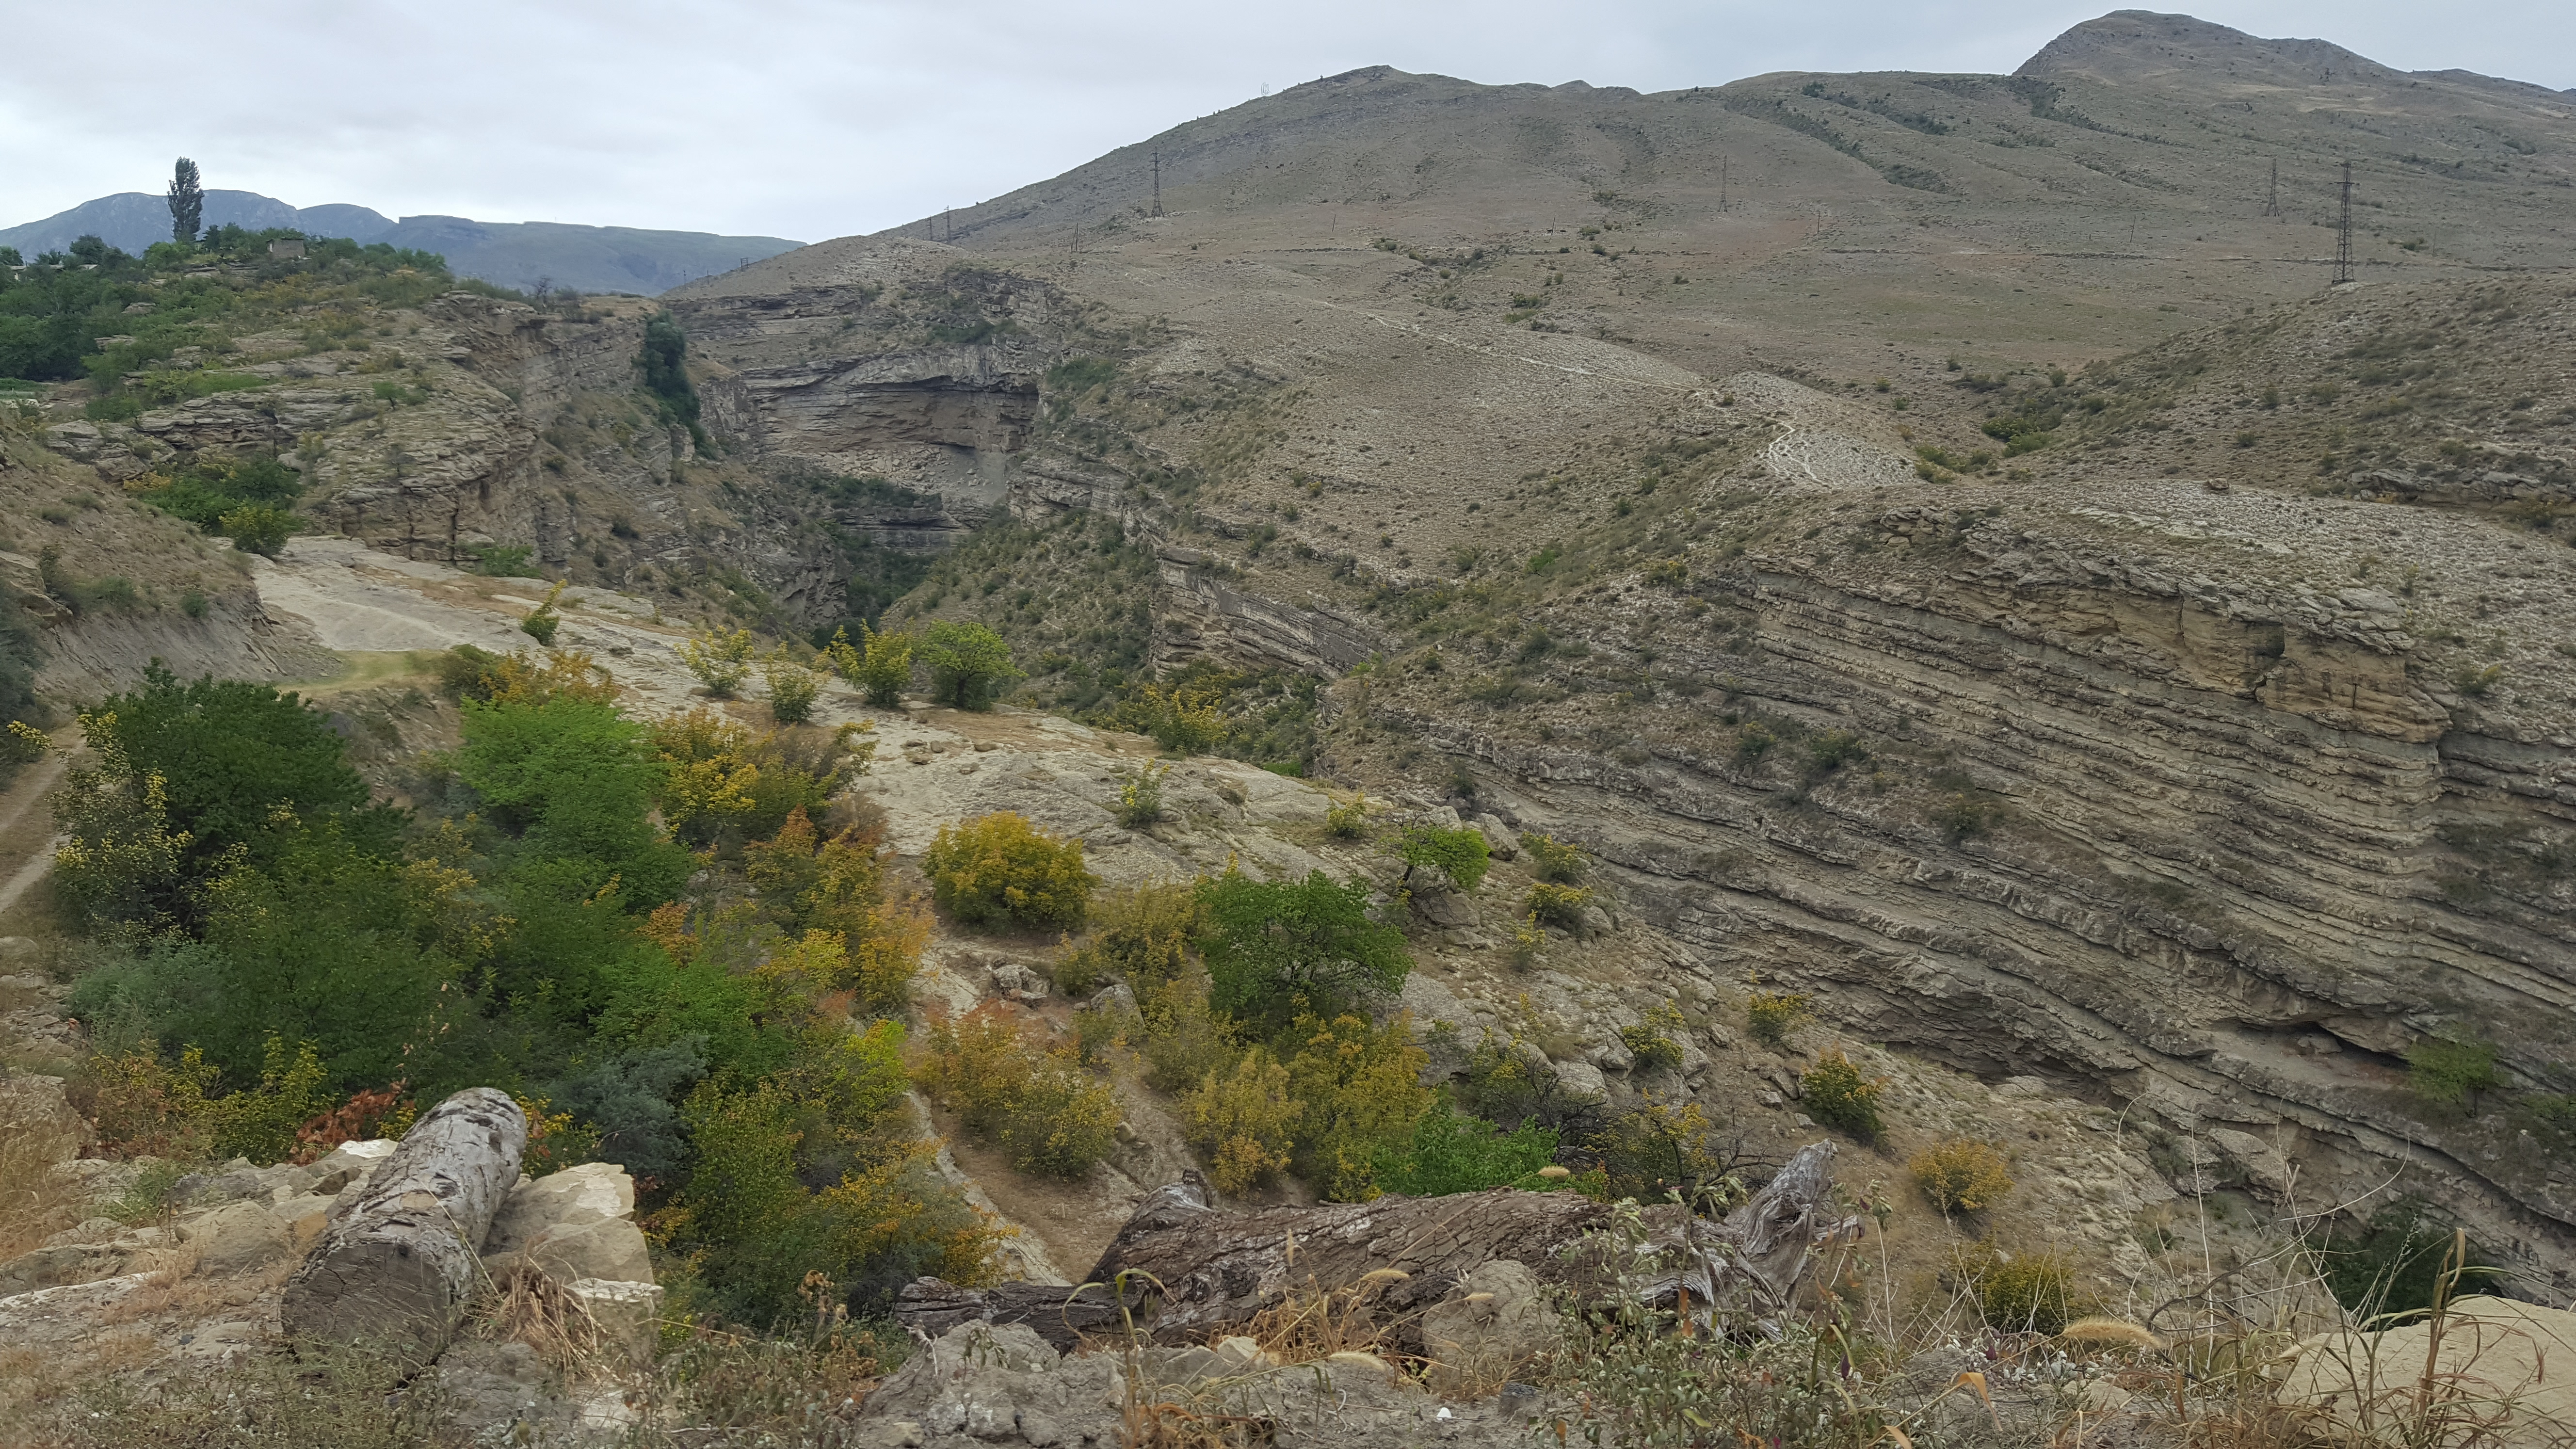
\includegraphics[height=6cm]{images/shajtane2.jpg}}
\end{figure}
\end{frame}

\begin{frame}{Shajt'ane}
\begin{figure}[h]
\centering
\fbox{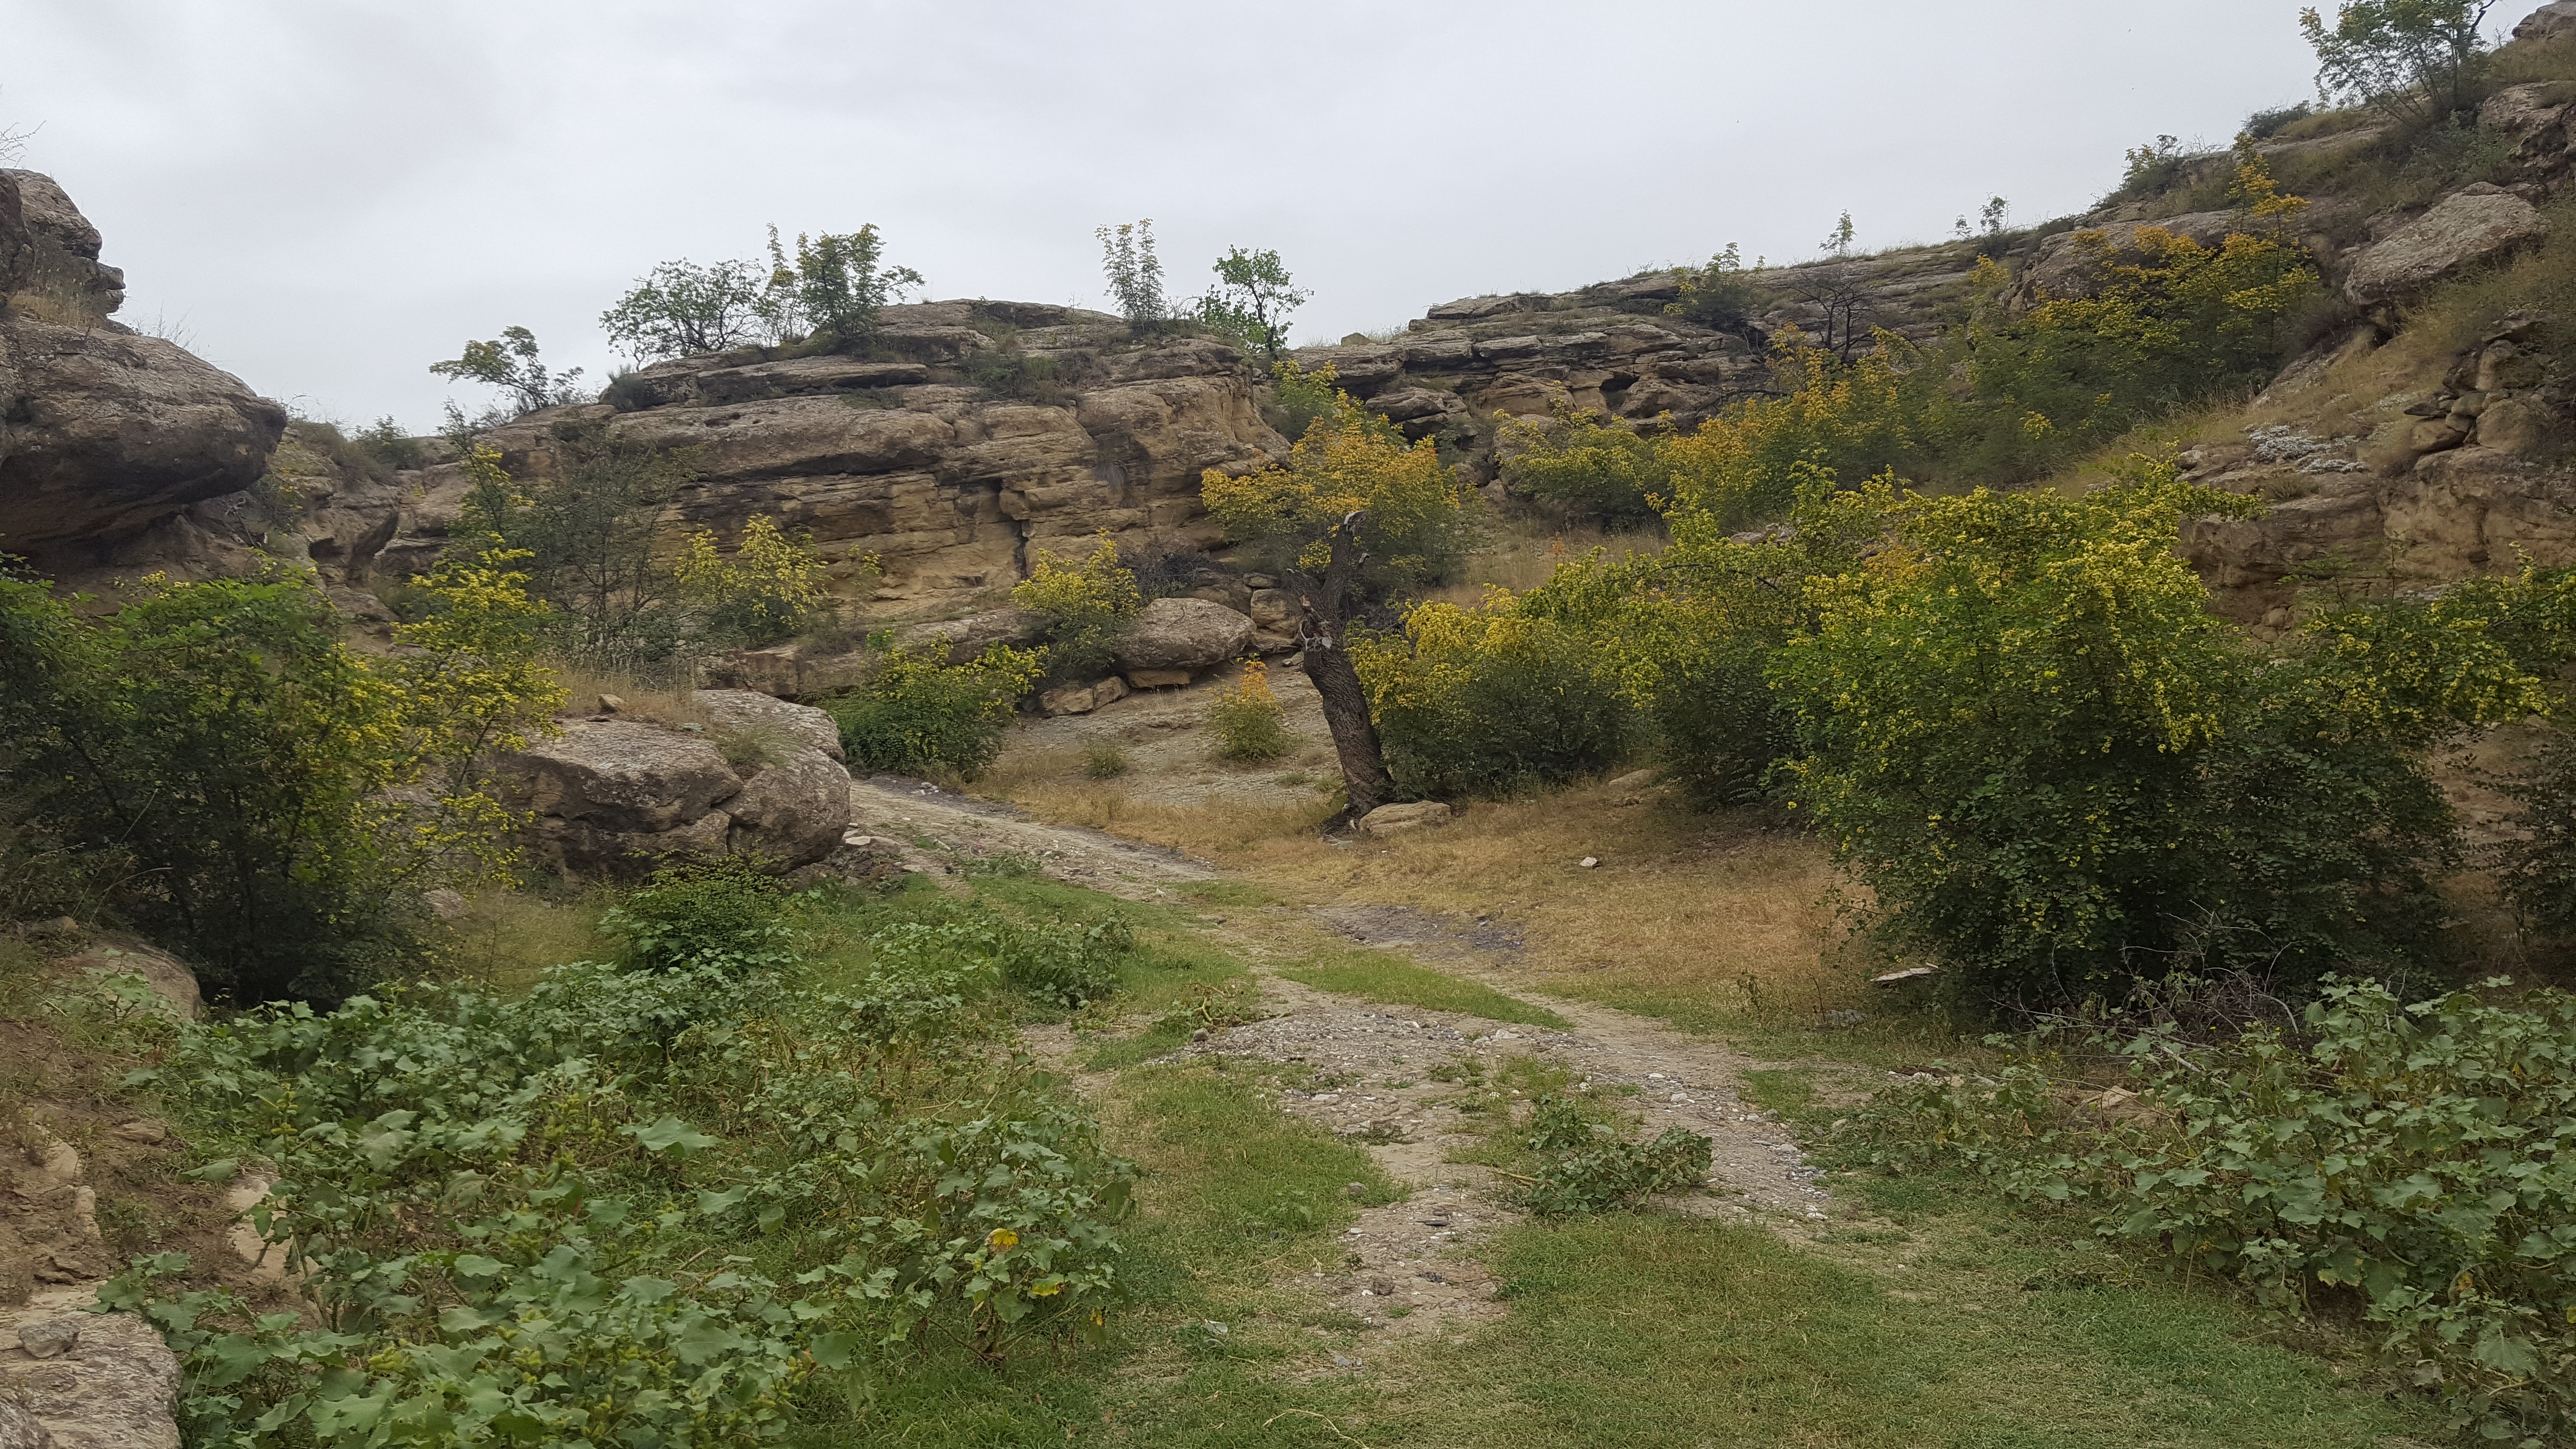
\includegraphics[height=6cm]{images/shajtane1.jpg}}
\end{figure}
\end{frame}

\begin{frame}{The mill}
\begin{figure}[h]
\centering
\fbox{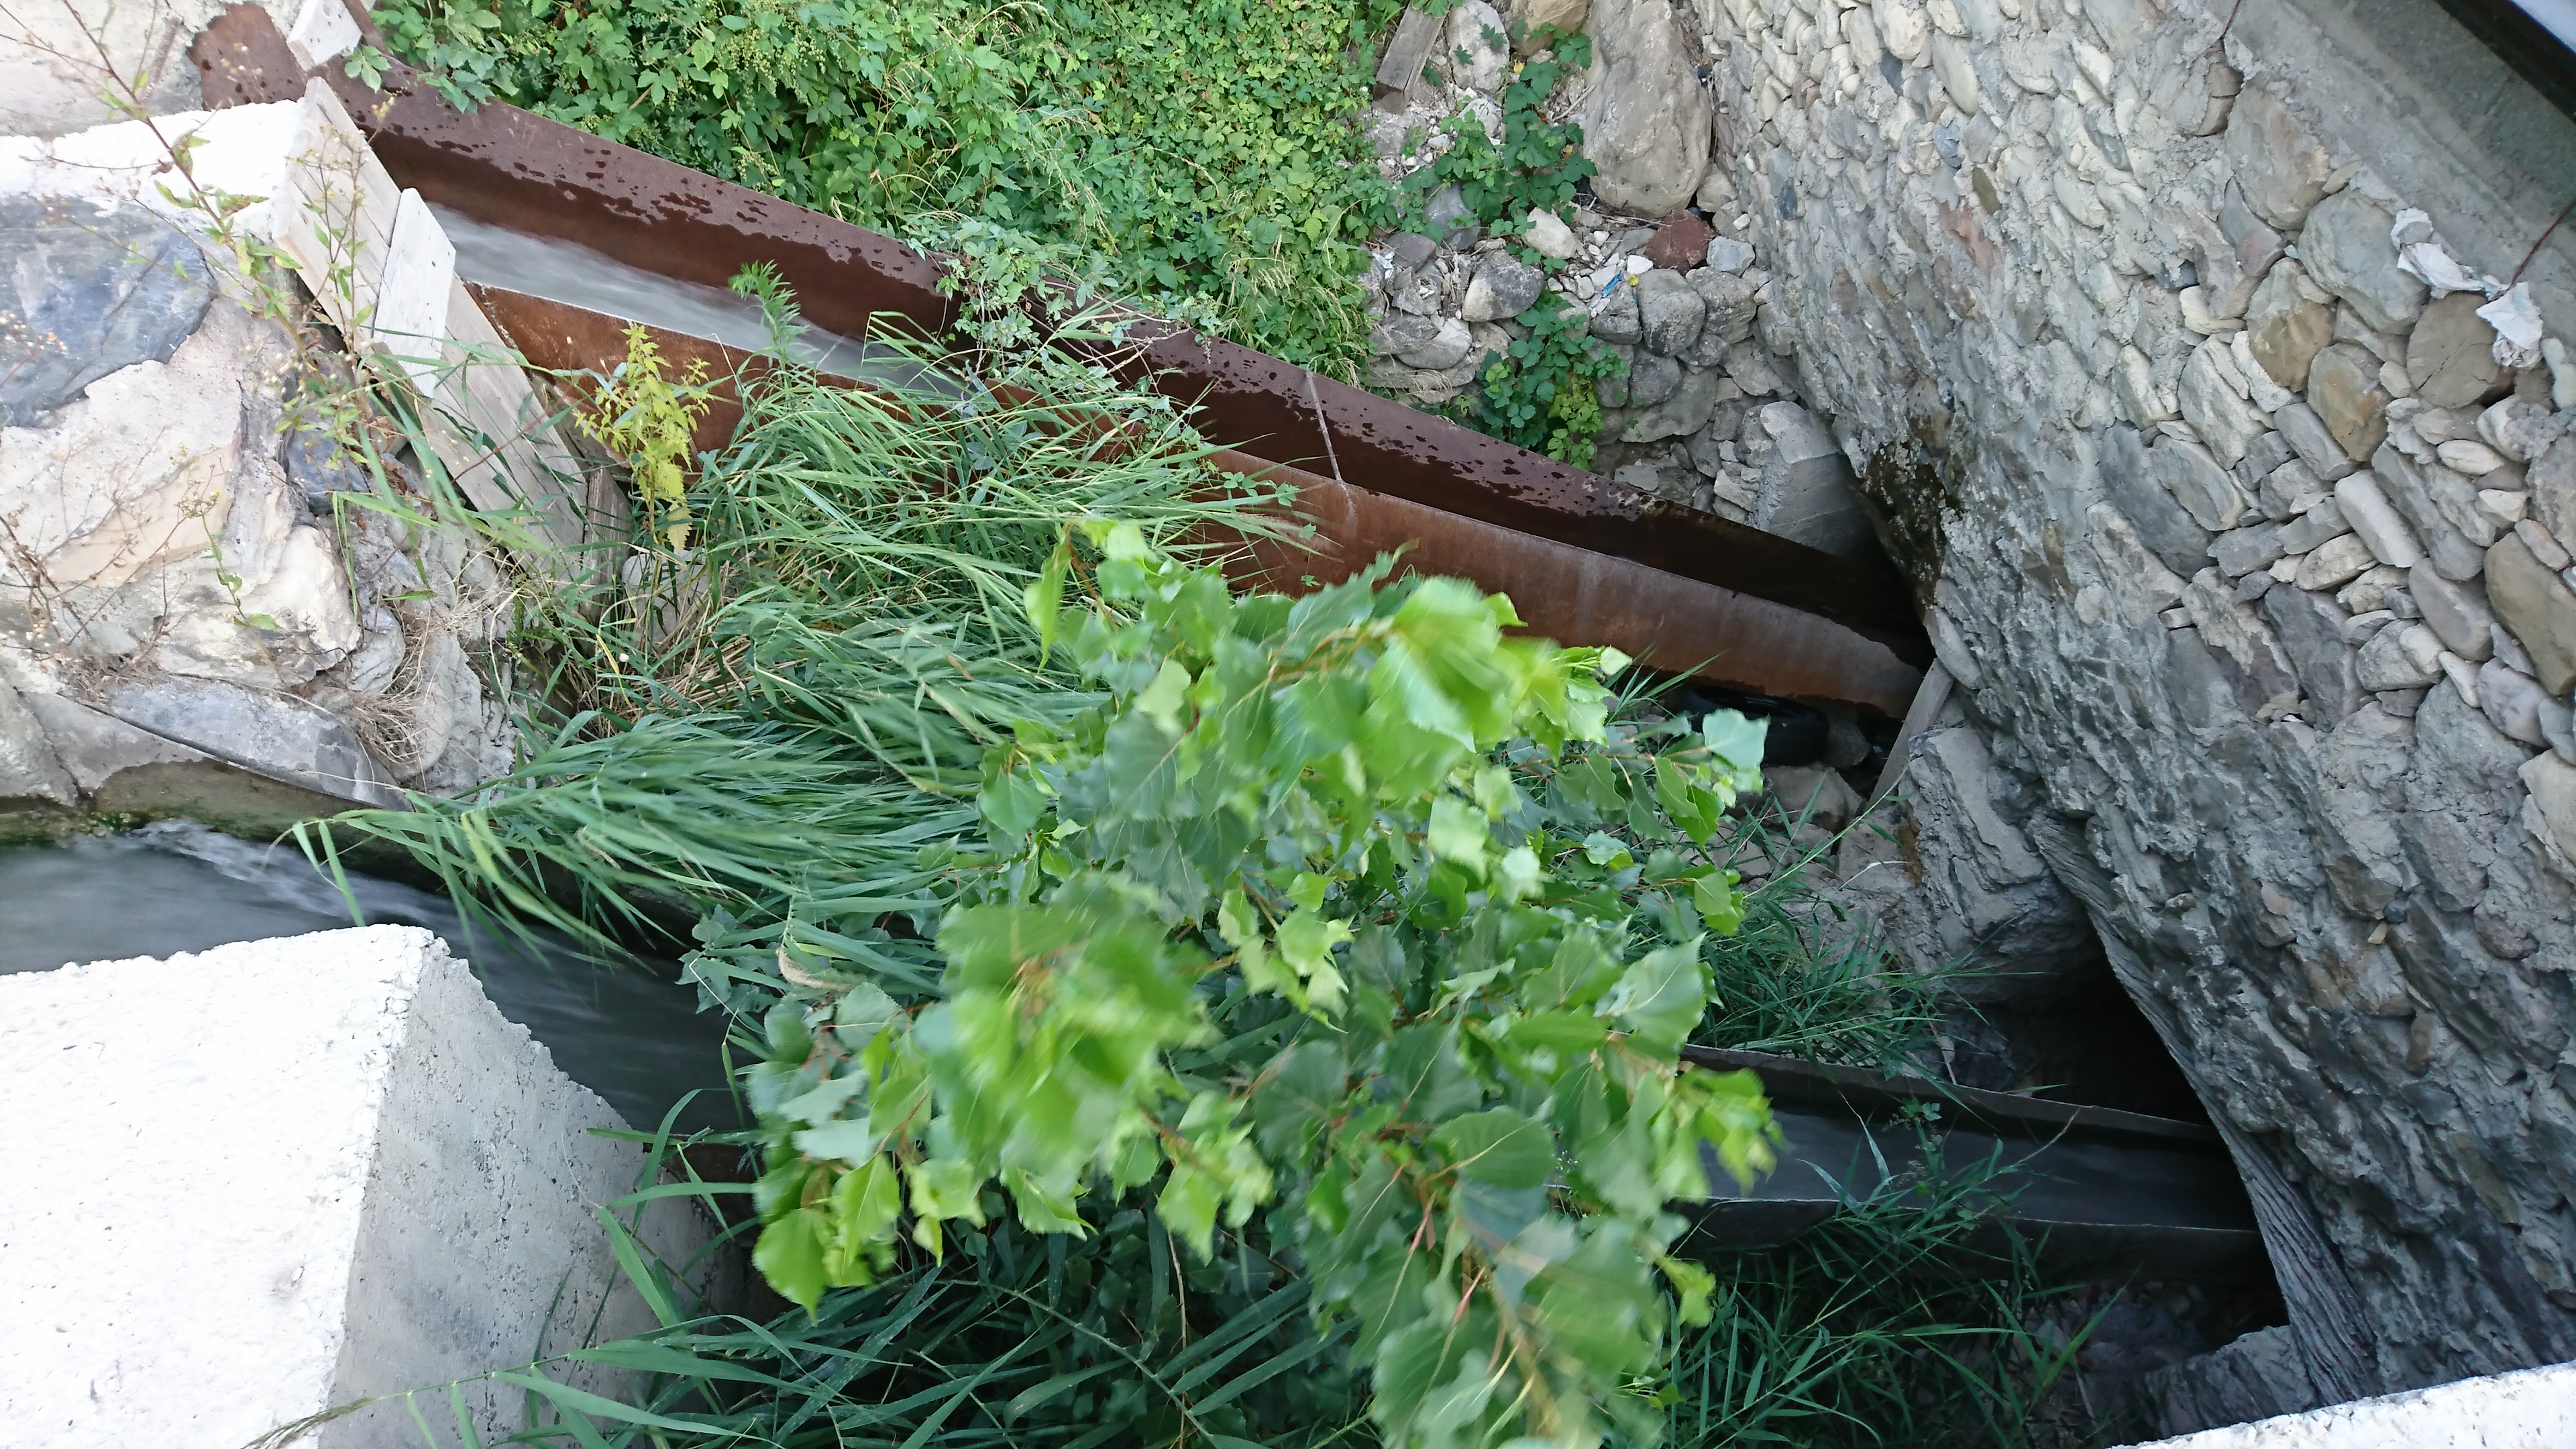
\includegraphics[height=6cm]{images/mill1.JPG}}
\end{figure}
\end{frame}

\begin{frame}{The mill}
\begin{figure}[h]
\centering
\fbox{\includegraphics[height=6cm]{images/mill2.JPG}}
\end{figure}
\end{frame}

\begin{frame}{Juice factory Ambré}
\begin{figure}[h]
\centering
\fbox{\includegraphics[height=6cm]{images/sok.JPG}}
\end{figure}
\end{frame}

\begin{frame}{The road to Makhachkala}
\begin{figure}[h]
\centering
\fbox{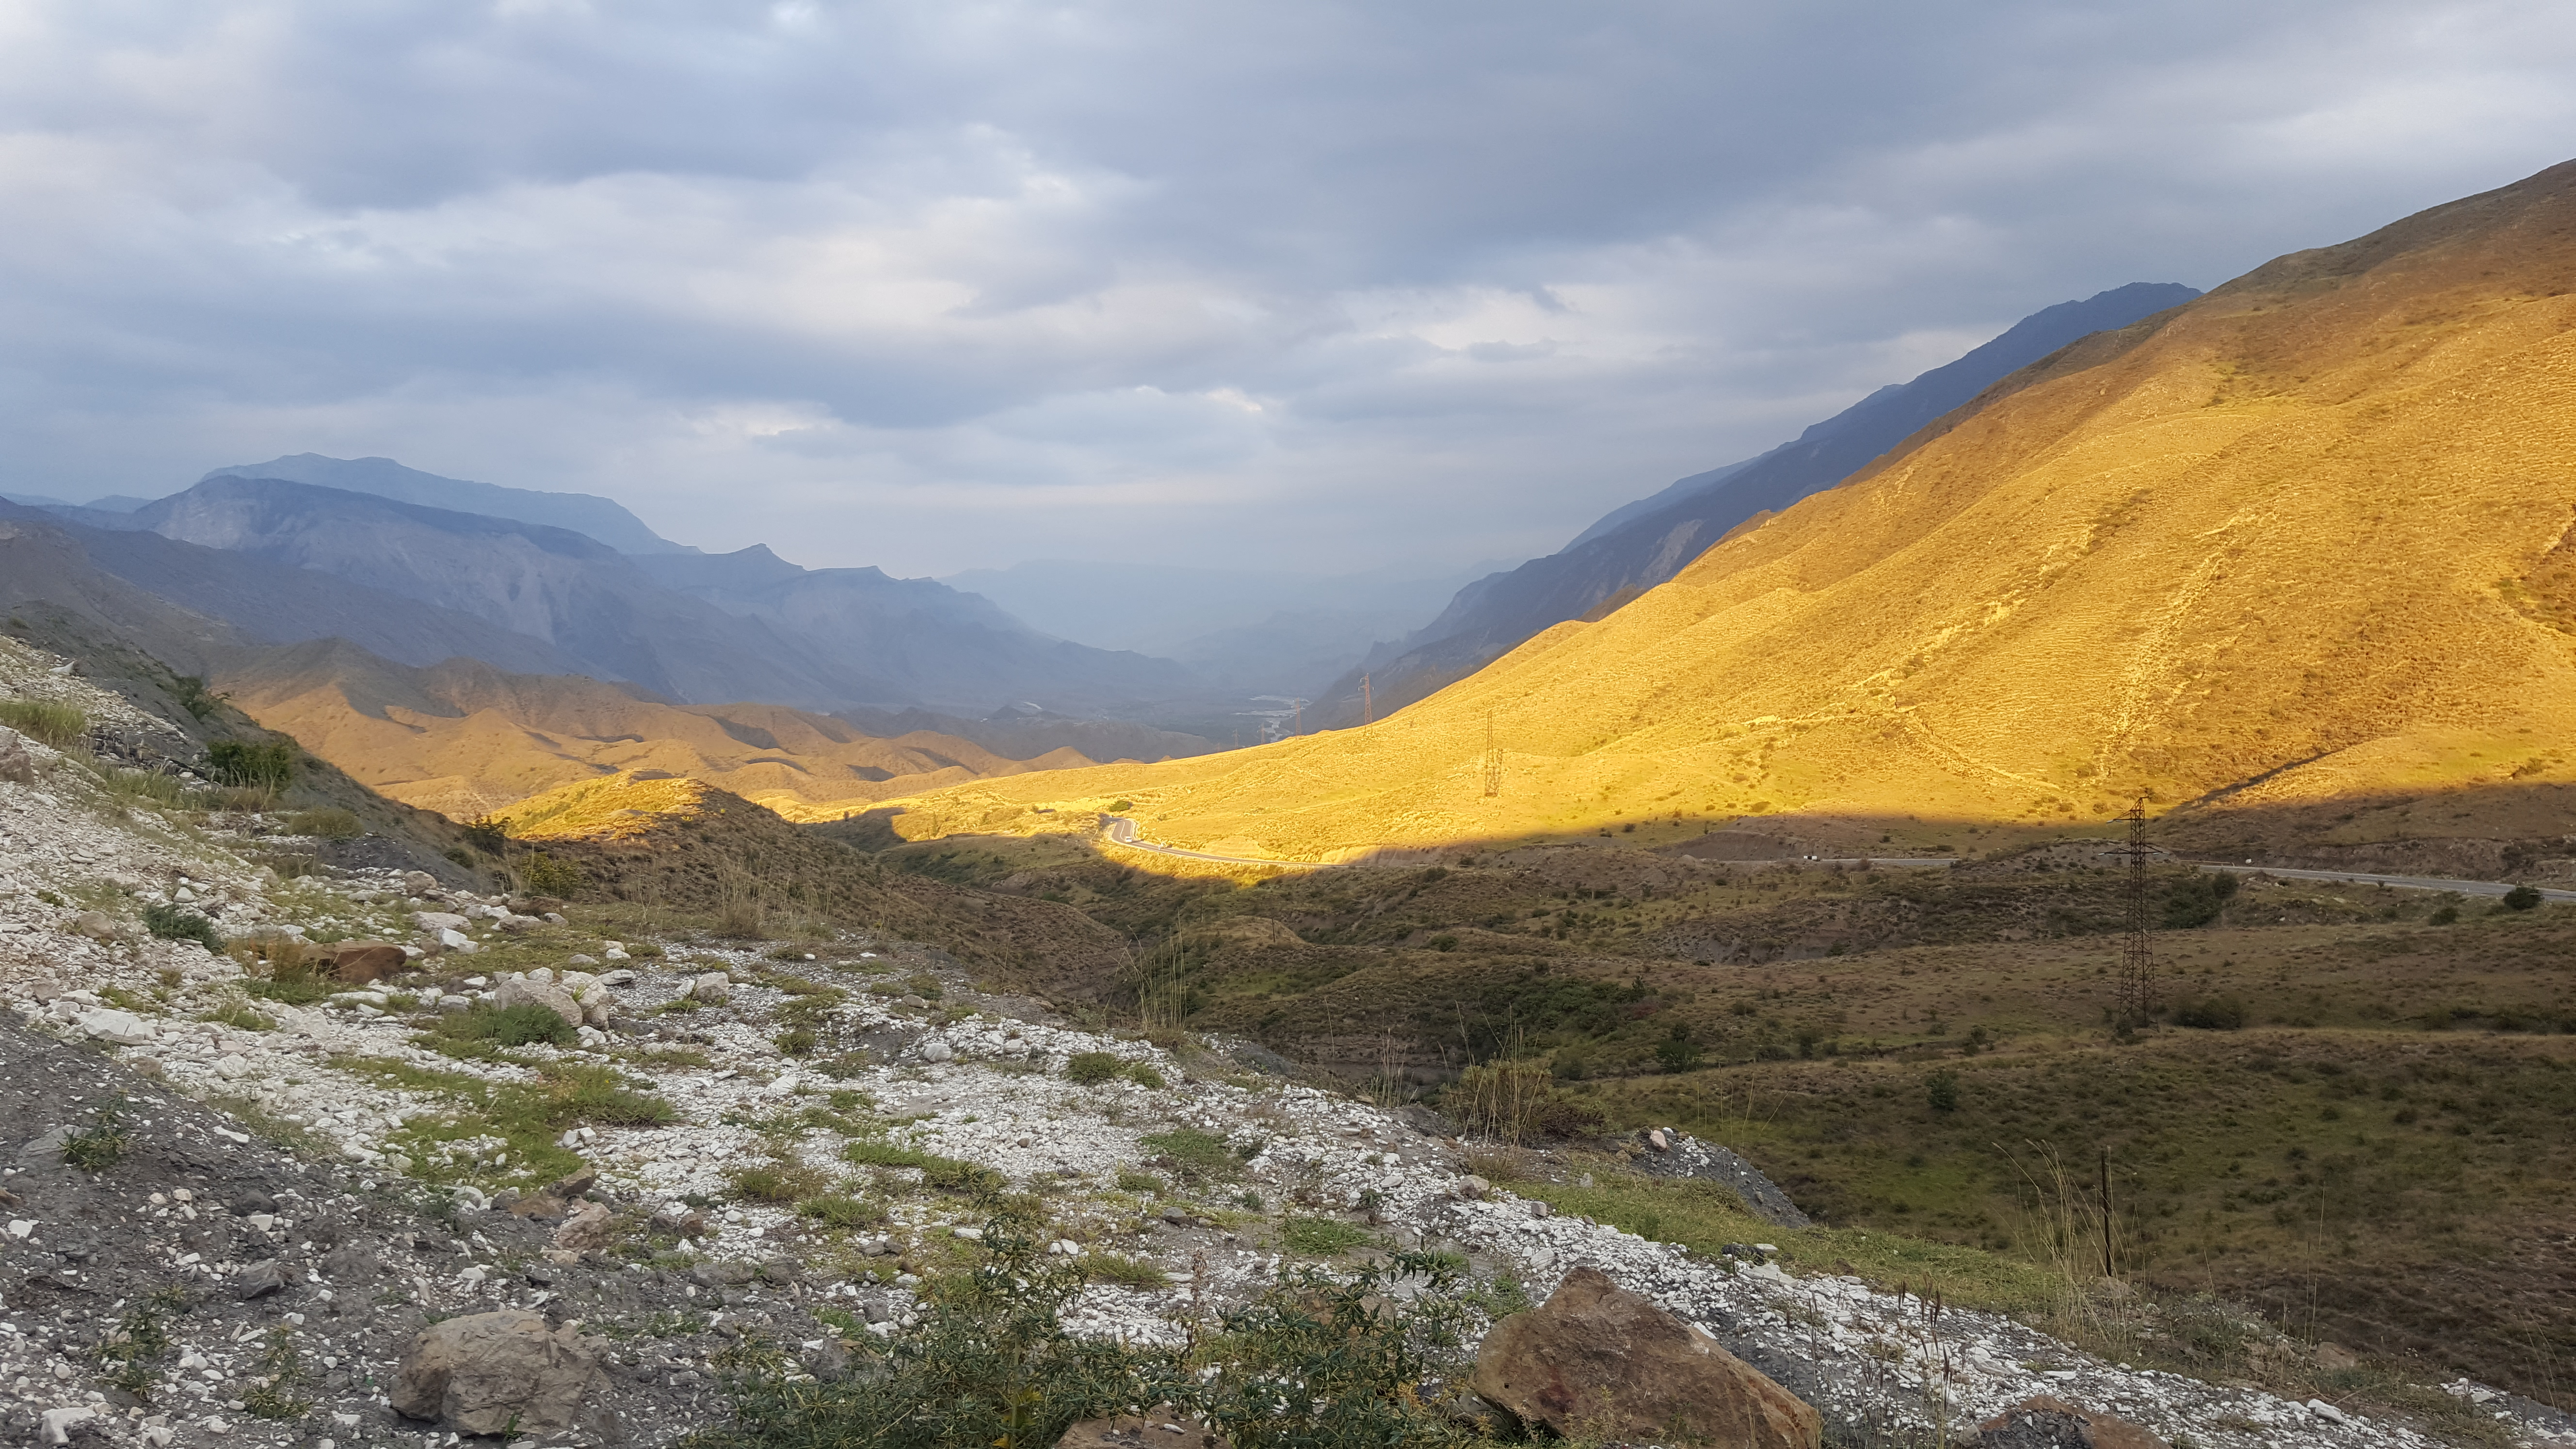
\includegraphics[height=6cm]{images/nice_picture.jpg}}
\end{figure}
\end{frame}

\begin{frame}{Бул1у. Спасибо!}
\begin{figure}[h]
\centering
\fbox{\includegraphics[height=6cm]{images/panorama.jpg}}
\end{figure}
\end{frame}

\section{Abbreviations}
\begin{frame}{Abbreviations}

\tiny{\printglossary}

\end{frame}

\section{References}
\begin{frame}{References}

\printbibliography

\end{frame}


\end{document}